\section{Design and Solution}

\subsection{System Overview}
The system is designed as an integrated hardware-software solution focusing on real-time signal processing. The core system architecture includes:

\subsubsection{Signal Processing Components}
\begin{itemize}
    \item ADC (12-bit resolution) for input signal capture
    \item DAC for scaled analog signal output
    \item TIM2 for precise frequency measurements
    \item GPIO for button input handling
    \item OLED Display for user interface
\end{itemize}

\subsubsection{Operational Modes}
\begin{itemize}
    \item \textbf{Function Generator Mode:} Displays measured frequency from the function generator
    \item \textbf{NE555 Timer Mode:} Display the 555 Timer Frequency
\end{itemize}

\subsubsection{System Integration}
\begin{itemize}
    \item Centralized control via STM32F051R8 microcontroller
    \item Interrupt-based event handling
    \item Real-time data processing pipeline
    \item User interface management
\end{itemize}

\noindent[0pt] The block diagram in Figure \ref{fig:systemoverview} The diagram illustrates the interconnections between various hardware modules and highlights the system's input, processing, and output stages, making it a typical system-level design representation for an embedded electronic device.

\begin{figure}[H]
    \centering
    \begin{tikzpicture}[
    node distance = 1cm,
    box/.style={
        draw=black,
        rectangle,
        minimum width=2.5cm,
        minimum height=1cm,
        align=center,
        rounded corners=3pt,
        fill=white,
        text=black,
        thick
    },
    group/.style={
        draw=black,
        rectangle,
        inner sep=0.5cm,
        rounded corners=5pt,
        thick
    },
    connection/.style={
        ultra thick,
        ->,
        >=stealth
    }
]

% External Components Group (Top Right)
\begin{scope}[xshift=12cm, local bounding box=ext]
    \node[box] (pot) at (0,0) {Potentiometer};
    \node[box] (adc_in) [right=1cm of pot] {ADC Input};
    
    \node[box] (ne555) [below=0.5cm of pot] {NE555 Timer};
    \node[box] (freq1) [right=1cm of ne555] {Frequency\\Input 1};
    
    \node[box] (fgen) [below=0.5cm of ne555] {Function\\Generator};
    \node[box] (freq2) [right=1cm of fgen] {Frequency\\Input 2};
    
    \node[box] (btn) [below=0.5cm of fgen] {Mode Button};
    \node[box] (btn_in) [right=1cm of btn] {Button Input};
    
    \node[group] (ext_group) [fit=(pot) (adc_in) (ne555) (freq1) (fgen) (freq2) (btn) (btn_in)] {};
    \node[above, font=\bfseries] at (ext_group.north) {External Components};
\end{scope}

% STM32F0 Core Group - Inputs (Top Left)
\begin{scope}[xshift=3cm, yshift=-2cm, local bounding box=inputs]
    \node[box] (adc) at (0,0) {ADC Module};
    \node[box] (tim) [below=0.5cm of adc] {Timer Module};
    \node[box] (exti) [below=0.5cm of tim] {External\\Interrupt};
    \node[group] (input_group) [fit=(adc) (tim) (exti)] {};
    \node[above, font=\bfseries] at (input_group.north) {Inputs};
\end{scope}

% Processing subgroup (Bottom Right)
\begin{scope}[xshift=7cm, yshift=-8cm, local bounding box=proc]
    \node[box] (cpu) at (0,0) {CPU Core};
    \node[box] (dac) [below=0.5cm of cpu] {DAC Module};
    \node[box] (disp) [below=0.5cm of dac] {Display\\Controller};
    \node[group] (proc_group) [fit=(cpu) (dac) (disp)] {};
    \node[above, font=\bfseries] at (proc_group.north) {Processing};
\end{scope}

% Draw Core group around both Input and Processing
\node[group] (core_group) [fit=(input_group) (proc_group)] {};
\node[above, font=\bfseries] at (core_group.north) {STM32F0 Core};

% Outputs Group (Bottom Left)
\begin{scope}[xshift=3cm, yshift=-8cm, local bounding box=out]
    \node[box] (ana_out) at (0,0) {Analog Output};
    \node[box] (oled) [below=0.5cm of ana_out] {OLED Display};
    \node[group] (out_group) [fit=(ana_out) (oled)] {};
    \node[above, font=\bfseries] at (out_group.north) {Outputs};
\end{scope}

% Connections with bend to avoid text
\draw[connection] (pot) -- (adc_in);
\draw[connection] (ne555) -- (freq1);
\draw[connection] (fgen) -- (freq2);
\draw[connection] (btn) -- (btn_in);

\draw[connection] (adc_in) to[bend right=30] (adc);
\draw[connection] (freq1) to[bend right=20] (tim);
\draw[connection] (freq2) to[bend right=15] (tim);
\draw[connection] (btn_in) to[bend right=10] (exti);

\draw[connection] (adc) to[bend right=10] (cpu);
\draw[connection] (tim) -- (cpu);
\draw[connection] (exti) to[bend left=10] (cpu);

\draw[connection] (cpu) -- (dac);
\draw[connection] (cpu) -- (disp);

\draw[connection] (dac) to[bend right=30] (ana_out);
\draw[connection] (disp) to[bend right=20] (oled);

\end{tikzpicture}
    \caption{STM32F0 Microcontroller System Block Diagram}
    \label{fig:systemoverview}
\end{figure}

% \begin{tikzpicture}[
    node distance = 1cm,
    box/.style={
        draw=black,
        rectangle,
        minimum width=2.5cm,
        minimum height=1cm,
        align=center,
        rounded corners=3pt,
        fill=white,
        text=black,
        thick
    },
    group/.style={
        draw=black,
        rectangle,
        inner sep=0.5cm,
        rounded corners=5pt,
        thick
    },
    connection/.style={
        ultra thick,
        ->,
        >=stealth
    }
]

% External Components Group (Top Right)
\begin{scope}[xshift=12cm, local bounding box=ext]
    \node[box] (pot) at (0,0) {Potentiometer};
    \node[box] (adc_in) [right=1cm of pot] {ADC Input};
    
    \node[box] (ne555) [below=0.5cm of pot] {NE555 Timer};
    \node[box] (freq1) [right=1cm of ne555] {Frequency\\Input 1};
    
    \node[box] (fgen) [below=0.5cm of ne555] {Function\\Generator};
    \node[box] (freq2) [right=1cm of fgen] {Frequency\\Input 2};
    
    \node[box] (btn) [below=0.5cm of fgen] {Mode Button};
    \node[box] (btn_in) [right=1cm of btn] {Button Input};
    
    \node[group] (ext_group) [fit=(pot) (adc_in) (ne555) (freq1) (fgen) (freq2) (btn) (btn_in)] {};
    \node[above, font=\bfseries] at (ext_group.north) {External Components};
\end{scope}

% STM32F0 Core Group - Inputs (Top Left)
\begin{scope}[xshift=3cm, yshift=-2cm, local bounding box=inputs]
    \node[box] (adc) at (0,0) {ADC Module};
    \node[box] (tim) [below=0.5cm of adc] {Timer Module};
    \node[box] (exti) [below=0.5cm of tim] {External\\Interrupt};
    \node[group] (input_group) [fit=(adc) (tim) (exti)] {};
    \node[above, font=\bfseries] at (input_group.north) {Inputs};
\end{scope}

% Processing subgroup (Bottom Right)
\begin{scope}[xshift=7cm, yshift=-8cm, local bounding box=proc]
    \node[box] (cpu) at (0,0) {CPU Core};
    \node[box] (dac) [below=0.5cm of cpu] {DAC Module};
    \node[box] (disp) [below=0.5cm of dac] {Display\\Controller};
    \node[group] (proc_group) [fit=(cpu) (dac) (disp)] {};
    \node[above, font=\bfseries] at (proc_group.north) {Processing};
\end{scope}

% Draw Core group around both Input and Processing
\node[group] (core_group) [fit=(input_group) (proc_group)] {};
\node[above, font=\bfseries] at (core_group.north) {STM32F0 Core};

% Outputs Group (Bottom Left)
\begin{scope}[xshift=3cm, yshift=-8cm, local bounding box=out]
    \node[box] (ana_out) at (0,0) {Analog Output};
    \node[box] (oled) [below=0.5cm of ana_out] {OLED Display};
    \node[group] (out_group) [fit=(ana_out) (oled)] {};
    \node[above, font=\bfseries] at (out_group.north) {Outputs};
\end{scope}

% Connections with bend to avoid text
\draw[connection] (pot) -- (adc_in);
\draw[connection] (ne555) -- (freq1);
\draw[connection] (fgen) -- (freq2);
\draw[connection] (btn) -- (btn_in);

\draw[connection] (adc_in) to[bend right=30] (adc);
\draw[connection] (freq1) to[bend right=20] (tim);
\draw[connection] (freq2) to[bend right=15] (tim);
\draw[connection] (btn_in) to[bend right=10] (exti);

\draw[connection] (adc) to[bend right=10] (cpu);
\draw[connection] (tim) -- (cpu);
\draw[connection] (exti) to[bend left=10] (cpu);

\draw[connection] (cpu) -- (dac);
\draw[connection] (cpu) -- (disp);

\draw[connection] (dac) to[bend right=30] (ana_out);
\draw[connection] (disp) to[bend right=20] (oled);

\end{tikzpicture}

\subsection{Hardware Design}

\subsubsection{Block Diagram}

The hardware architecture (Figure \ref{fig:systemblocks}) consists of the following interconnected components:
\begin{itemize}
    \item STM32F051R8 microcontroller (central processor)
    \item Input devices (potentiometer, function generator)
    \item Output devices (DAC, OLED display)
    \item Control interfaces (mode-switch button)
\end{itemize}

\begin{figure}[H]
    \centering
    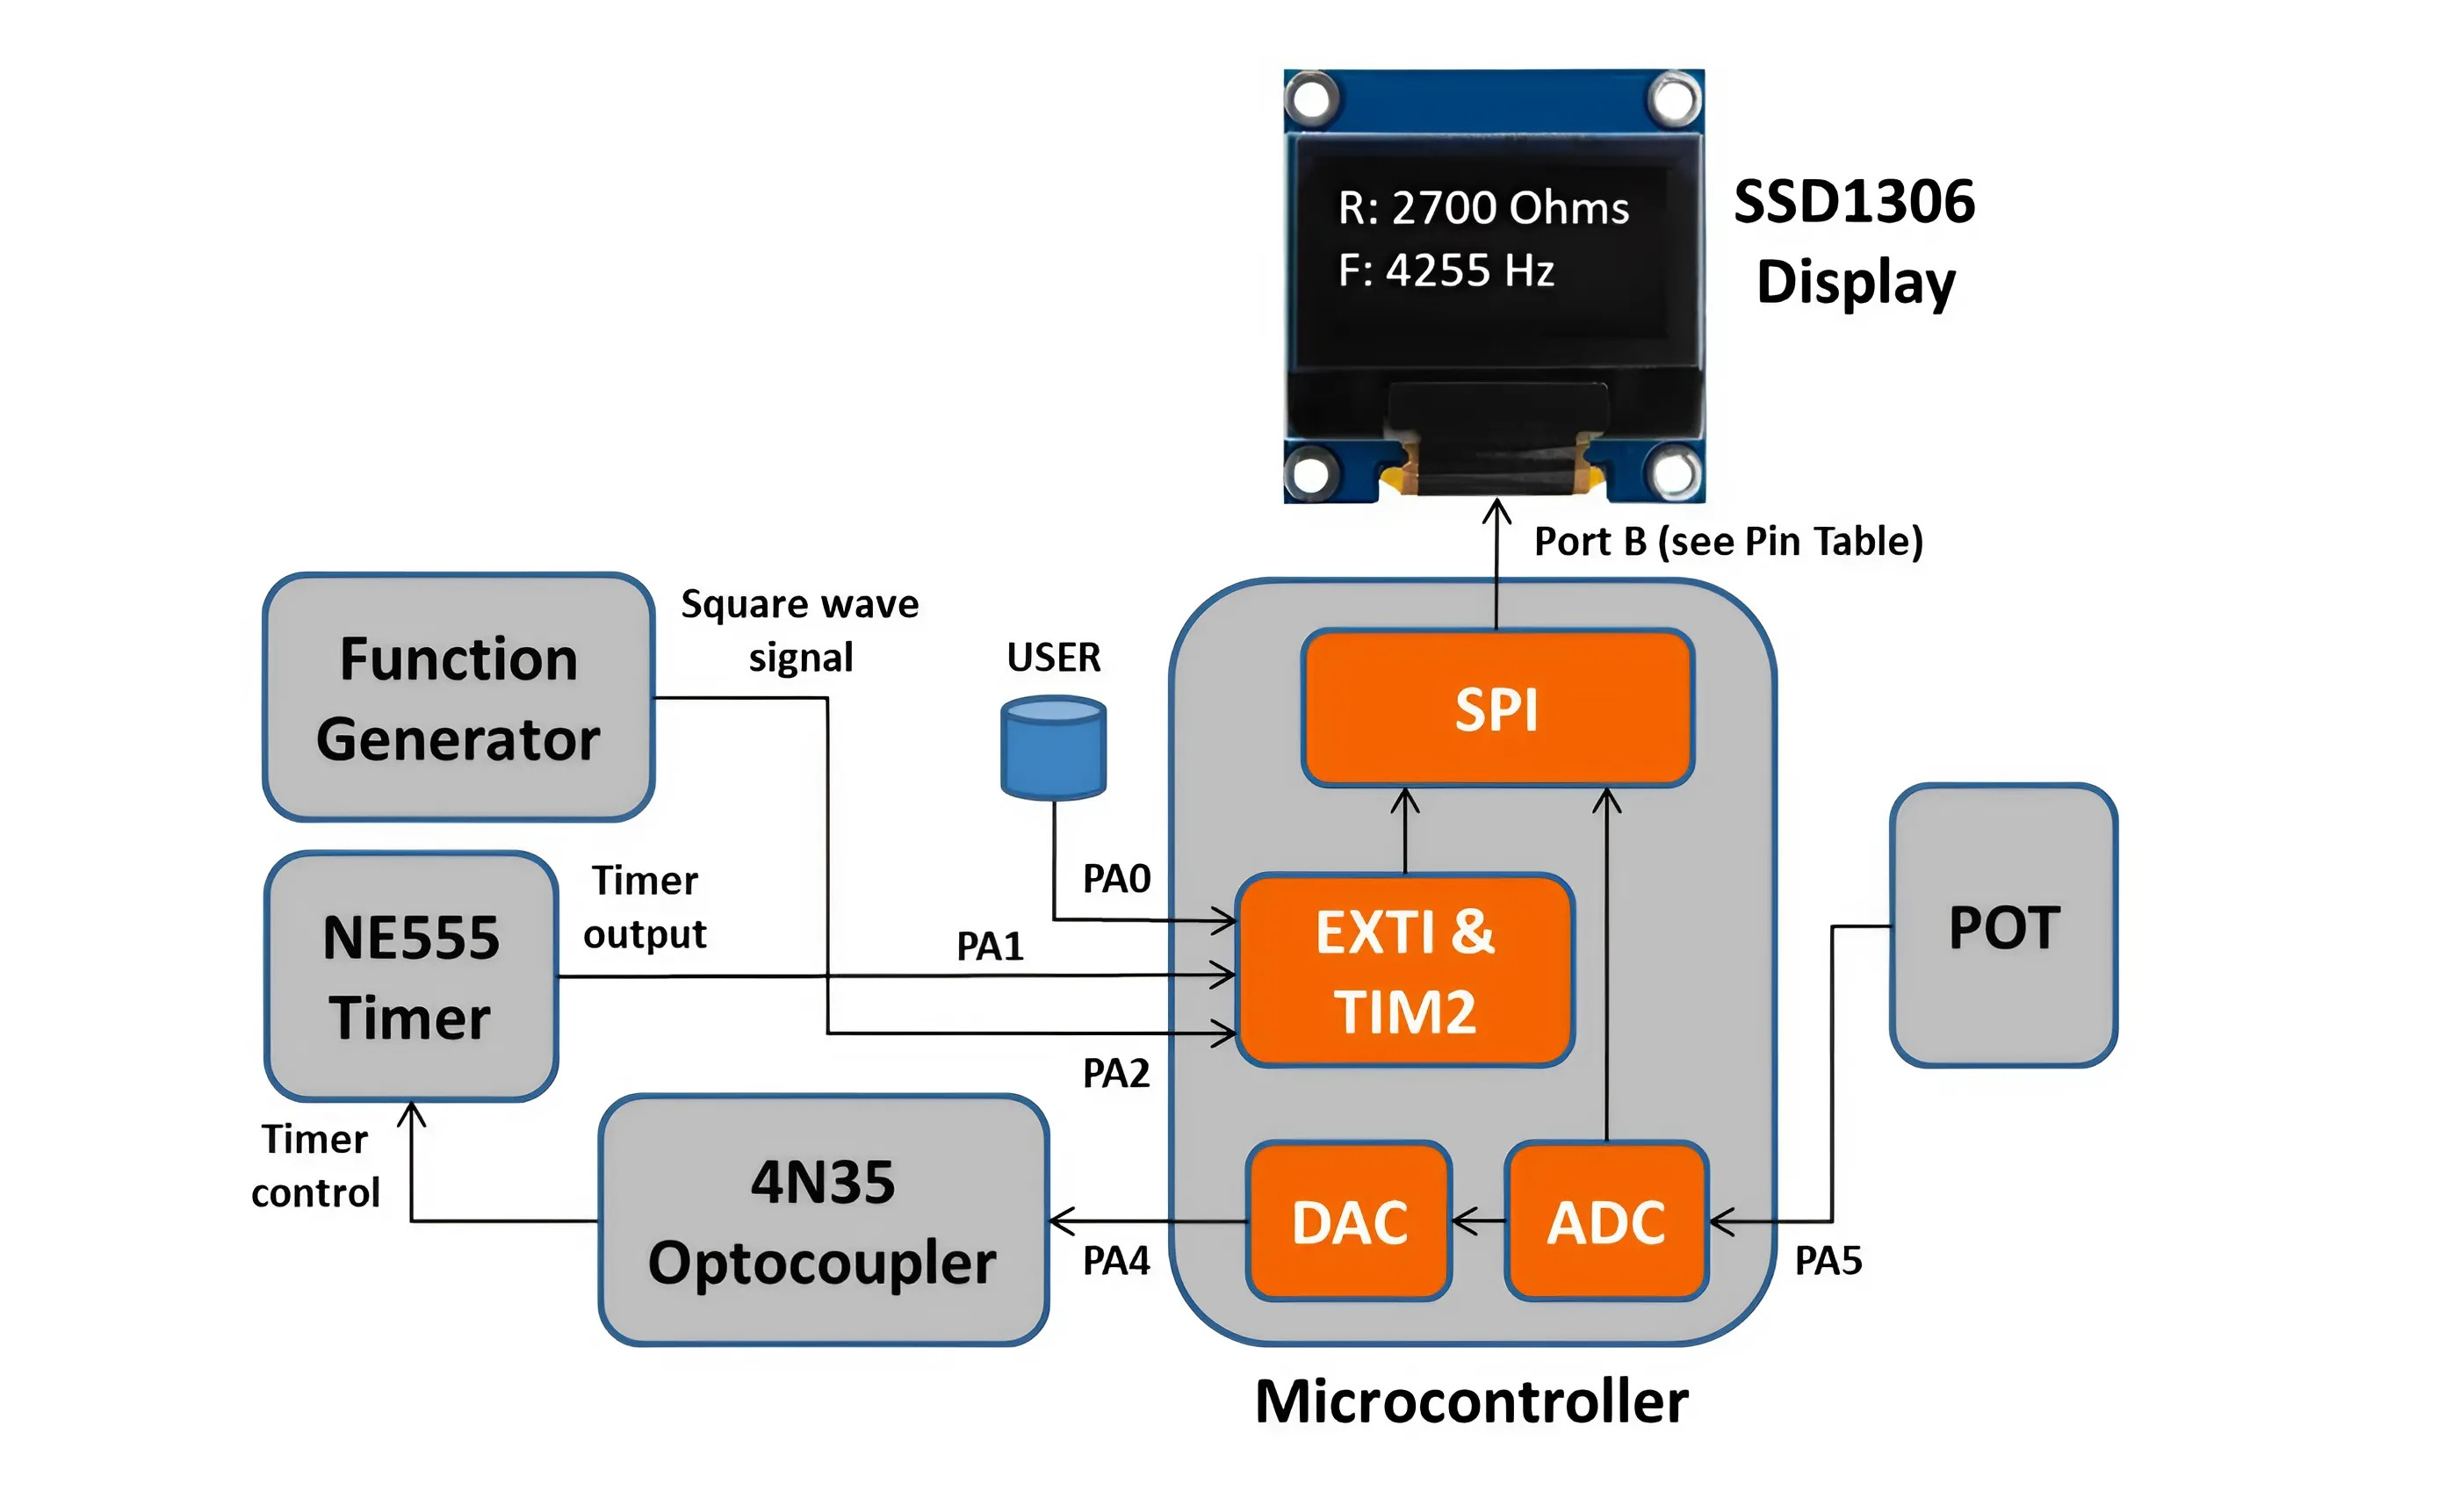
\includegraphics[width=0.7\linewidth]{graphics/system_blocks}
    \caption{System architecture showing the interaction between major components of the frequency measurement and signal generation system \cite{lab-manual}}
    \label{fig:systemblocks}
\end{figure}

\subsubsection{Hardware Components~\cite{lab-manual}}
\begin{itemize}
    \item \textbf{STM32F051R8 Microcontroller:} Central processing unit
    \item \textbf{Potentiometer:} Analog input source
    \item \textbf{OLED Display (SSD1306):} User interface display
    \item \textbf{Mode-Switch Button:} System control
    \item \textbf{Passive Components:} Signal conditioning
\end{itemize}

\subsubsection{Pin Configuration~\cite{lab-manual}}
\begin{itemize}
     \item PA0: USER button interrupt handling (EXTI0) 
     \item PA1: NE555 timer signal measurement (EXTI1)
     \item PA2: Function generator frequency measurement (EXTI2)
    \item PA4: DAC output for optocoupler control
    \item PA5: ADC input for potentiometer measurement
    \item PB3-PB7: SPI and control signals for OLED display
\end{itemize}

\begin{figure}[H]
    \centering
    \begin{tikzpicture}[
    node distance = 2cm,
    box/.style={
        draw=black,
        rectangle,
        minimum width=2cm,
        align=center,
        rounded corners=3pt,
        fill=white,
        text=black,
        thick
    },
    group/.style={
        draw=black,
        rectangle,
        inner sep=0.5cm,
        rounded corners=5pt,
        thick
    },
    connection/.style={
        ultra thick,
        ->,
        >=stealth
    }
]

% Calculate total height for vertical centering
\def\totalheight{7cm}  % Approximate height of the boxes

% STM32F0 Group
\begin{scope}[local bounding box=stm]
    \node[box] (pa0) at (0,\totalheight/2) {PA0:\\ Mode Button};
    \node[box] (pa1) [below=0.5cm of pa0] {PA1:\\ NE555 Input};
    \node[box] (pa2) [below=0.5cm of pa1] {PA2:\\ FGen Input};
    \node[box] (pa4) [below=0.5cm of pa2] {PA4:\\ DAC Output};
    \node[box] (pa5) [below=0.5cm of pa4] {PA5:\\ ADC Input};
    \node[box] (pb3) [below=0.5cm of pa5] {PB3:\\ OLED SCLK Output};
    \node[box] (pb4) [below=0.5cm of pb3] {PB4:\\ OLED RES\# Output};
    \node[box] (pb5) [below=0.5cm of pb4] {PB5:\\ OLED SDIN Output};
    \node[box] (pb6) [below=0.5cm of pb5] {PB6:\\ OLED CS\# Output};
    \node[box] (pb7) [below=0.5cm of pb6] {PB7:\\ OLED D/C\# Output};
    \node[group] (stm32) [fit=(pa0) (pa1) (pa2) (pa4) (pa5) (pb3) (pb4) (pb5) (pb6) (pb7)] {};
    \node[above, font=\bfseries] at (stm32.north) {STM32F0};
\end{scope}

% Features Group
\begin{scope}[xshift=6cm, local bounding box=feat]  % Increased xshift
    \node[box] (dig) at (0,\totalheight/2) {Digital Input Mode};
    \node[box] (freq1) [below=0.5cm of dig] {Frequency Input Mode};
    \node[box] (freq2) [below=0.5cm of freq1] {Frequency Input Mode};
    \node[box] (anaout) [below=0.5cm of freq2] {Analog Output Mode};
    \node[box] (anain) [below=0.5cm of anaout] {Analog Input Mode};
    \node[box] (screenout) [below=0.5cm of anain] {Screen Output Mode};
    \node[box] (screenout2) [below=0.5cm of screenout] {Screen Output Mode};
    \node[group] (features) [fit=(dig) (freq1) (freq2) (anaout) (anain) (screenout) (screenout2)] {};
    \node[above, font=\bfseries] at (features.north) {Features};
\end{scope}

% Characteristics Group
\begin{scope}[xshift=12cm, local bounding box=char]  % Increased xshift
    \node[box] (btnchar) at (0,\totalheight/2) {Pull-up enabled\\ EXTI enabled};
    \node[box] (freq1char) [below=0.5cm of btnchar] {No pull-up/down\\ EXTI enabled};
    \node[box] (freq2char) [below=0.5cm of freq1char] {No pull-up/down\\ EXTI enabled};
    \node[box] (dacchar) [below=0.5cm of freq2char] {12-bit resolution\\ 0.126-2.23V range};
    \node[box] (adcchar) [below=0.5cm of dacchar] {12-bit resolution\\ 0-3.3V range};
    \node[box] (output) [below=0.5cm of adcchar] {No pull-up/down\\ Alternate function};
    \node[box] (afoutput) [below=0.5cm of output] {No pull-up/down\\ Push-pull output type};
    \node[group] (chars) [fit=(btnchar) (freq1char) (freq2char) (dacchar) (adcchar) (output) (afoutput)] {};
    \node[above, font=\bfseries] at (chars.north) {Characteristics};
\end{scope}

% Connections with distinct colors
\draw[connection, blue] (pa0) -- (dig);
\draw[connection, red] (pa1) -- (freq1);
\draw[connection, green!50!black] (pa2) -- (freq2);
\draw[connection, orange] (pa4) -- (anaout);
\draw[connection, purple] (pa5) -- (anain);
\draw[connection, magenta] (pb3) -- (screenout);
\draw[connection, magenta] (pb5) -- (screenout);
\draw[connection, cyan] (pb4) -- (screenout2);
\draw[connection, cyan] (pb6) -- (screenout2);
\draw[connection, cyan] (pb7) -- (screenout2);

\draw[connection, blue] (dig) -- (btnchar);
\draw[connection, red] (freq1) -- (freq1char);
\draw[connection, green!50!black] (freq2) -- (freq2char);
\draw[connection, orange] (anaout) -- (dacchar);
\draw[connection, purple] (anain) -- (adcchar);
\draw[connection, magenta] (screenout) -- (output);
\draw[connection, cyan] (screenout2) -- (afoutput);

\end{tikzpicture}
    \caption{Pin Configurations of the GPIO Pins \cite{lab-manual}}
    \label{fig:pinconfig}
\end{figure}

\subsubsection{Power Distribution}
\begin{itemize}
    \item Main supply: 3.3 V Power Supply (Allowable $V_{DD}$: 2.0 to 3.6 V \cite{stm32-datasheet})
    \item Separate analog/digital grounds
    \item Decoupling capacitors for noise reduction
\end{itemize}

\newpage

\section{Software Design}
The software is designed with the intent of maintainability and debugging. However, there is room for improvement in modularization (except for the OLED screen) to better achieve these goals. Key initialization functions and operational logic are outlined below.

\subsection{Initialization Functions}
The examples of the initialization functions from the project configure the system's peripherals, including the GPIO, ADC, DAC, and timers. (See Appendices \ref{sec:main_c} and \ref{sec:oled_screen_c} for the full code.)

\subsubsection{System Clock}
\begin{lstlisting}[caption=System Clock Initialization Function \cite{iox}]
void SystemClock48MHz(void) {
    // Disable the PLL
    RCC->CR &= ~(RCC_CR_PLLON);
    // Wait for the PLL to unlock
    while ((RCC->CR & RCC_CR_PLLRDY) != 0);
    // Configure the PLL for a 48 MHz system clock
    RCC->CFGR = 0x00280000;
    // Enable the PLL
    RCC->CR |= RCC_CR_PLLON;
    // Wait for the PLL to lock
    while ((RCC->CR & RCC_CR_PLLRDY) != RCC_CR_PLLRDY);
    // Switch to the PLL as the clock source
    RCC->CFGR = (RCC->CFGR & (~RCC_CFGR_SW_Msk)) | RCC_CFGR_SW_PLL;
    // Update the system clock variable
    SystemCoreClockUpdate();
}
\end{lstlisting}

\subsubsection{GPIO Initialization}
\begin{lstlisting}[caption=GPIO Port A Initialization Function \cite{iox}]
void myGPIOA_Init(void) {
    // Enable GPIOA clock
    RCC->AHBENR |= RCC_AHBENR_GPIOAEN;
    
    // Configure PA0 (button) as input
    GPIOA->MODER &= ~(GPIO_MODER_MODER0);
    
    // Configure PA1 (555 timer) as input
    GPIOA->MODER &= ~(GPIO_MODER_MODER1);
    
    // Configure PA2 (function generator) as input
    GPIOA->MODER &= ~(GPIO_MODER_MODER2);
    
    // Configure PA4 and PA5 as analog mode
    GPIOA->MODER |= GPIO_MODER_MODER4;
    GPIOA->MODER |= GPIO_MODER_MODER5;
    
    // Ensure no pull-up/pull-down for PA1 and PA2
    GPIOA->PUPDR &= ~(GPIO_PUPDR_PUPDR1 | GPIO_PUPDR_PUPDR2);
}
\end{lstlisting}


\subsubsection{ADC and DAC Initialization}
\begin{lstlisting}[caption=ADC and DAC Initialization Function \cite{interfacex}]
void myADC_Init(void) {
    // Enable ADC clock
    RCC->APB2ENR |= RCC_APB2ENR_ADC1EN;
    
    // Configure ADC settings
    ADC1->SMPR = 0x7;                // Maximum sampling time
    ADC1->CHSELR = ADC_CHSELR_CHSEL5;// Select channel 5
    
    // Calibrate ADC if enabled
    if (ENABLE_CAL) {
        ADC1->CR = ADC_CR_ADCAL;
        while (ADC1->CR == ADC_CR_ADCAL);
    }
    
    // Enable ADC and wait for ready
    ADC1->CR |= ADC_CR_ADEN;
    while (!(ADC1->ISR & ADC_ISR_ADRDY));
    
    // Configure continuous conversion mode
    ADC1->CFGR1 |= (ADC_CFGR1_CONT | ADC_CFGR1_OVRMOD);
}

void myDAC_init(void) {
    // Enable DAC Clock
    RCC->APB1ENR |= RCC_APB1ENR_DACEN;
    
    // Clear and configure DAC control register
    DAC->CR &= ~(0x7);
    DAC->CR |= DAC_CR_EN1;
}
\end{lstlisting}

\subsubsection{Timer (TIM2) Initialization}
\begin{lstlisting}[caption=Timer 2 Initialization Function \cite{iox}]
void myTIM2_Init(void) {
    // Enable clock for TIM2
    RCC->APB1ENR |= RCC_APB1ENR_TIM2EN;
    
    // Configure TIM2
    TIM2->CR1 = ((uint16_t)0x008C);
    TIM2->PSC = myTIM2_PRESCALER;
    TIM2->ARR = myTIM2_PERIOD;
    
    // Update timer registers
    TIM2->EGR |= ((uint16_t)0x0001);
    
    // Configure and enable interrupts
    NVIC_SetPriority(TIM2_IRQn, 0);
    NVIC_EnableIRQ(TIM2_IRQn);
    TIM2->DIER |= TIM_DIER_UIE;
}
\end{lstlisting}

\subsubsection{External Interrupt Initialization}
\begin{lstlisting}[caption=EXTI Initialization Function \cite{iox}]
void EXTI_Init(void) {
    // Map EXTI2 and EXTI0 lines to PA2 and PA0 respectively
    SYSCFG->EXTICR[0] &= ~(SYSCFG_EXTICR1_EXTI0 | SYSCFG_EXTICR1_EXTI1 | SYSCFG_EXTICR1_EXTI2);
    SYSCFG->EXTICR[0] |= (SYSCFG_EXTICR1_EXTI0_PA | SYSCFG_EXTICR1_EXTI1_PA | SYSCFG_EXTICR1_EXTI2_PA);

    // Set rising-edge trigger for EXTI2 and EXTI0 lines
    EXTI->RTSR |= (EXTI_RTSR_TR0 | EXTI_RTSR_TR1 | EXTI_RTSR_TR2);

    // Unmask interrupts from EXTI2 and EXTI0 lines
    EXTI->IMR |= (EXTI_IMR_IM0 | EXTI_IMR_IM1);

    // Configure interrupt priorities and enable in NVIC
    NVIC_SetPriority(EXTI0_1_IRQn, 0);
    NVIC_EnableIRQ(EXTI0_1_IRQn);

    NVIC_SetPriority(EXTI2_3_IRQn, 1);
    NVIC_EnableIRQ(EXTI2_3_IRQn);
}
\end{lstlisting}

\subsection{Core Logic}

\subsubsection{Signal Measurement and Reconstruction}
\begin{lstlisting}[caption=ADC Reading and DAC Writing Function \cite{interfacex}]
// ADC Reading (Measurement)
uint32_t readADC(void) {
    // Start ADC conversion
    ADC1->CR |= ADC_CR_ADSTART;
    
    // Wait for conversion completion
    while (!(ADC1->ISR & ADC_ISR_EOC));
    
    // Return the ADC result
    return ADC1->DR;
}

// Write to DAC (Reconstruction)
void writeDAC(uint32_t adc_val)
{
	// DHR12R1 is the 12-bit right-aligned data
	DAC->DHR12R1 = adc_val;
}
\end{lstlisting}

\subsubsection{Frequency and Resistance Computation}
\begin{lstlisting}[caption=Frequency and Resistance Computation]
void measure_frequency(unsigned int bit_number, unsigned int* var_address) {
    // Assign some necessary variables
    unsigned int count = 0;
    float period = 0;
    float frequency = 0;
    // Compute the register mask by bit number
    uint32_t register_mask = EXTI_PR_PR0 << bit_number;

    /* Check if EXTI2 interrupt pending flag is indeed set */
    if ((EXTI->PR & register_mask) != 0) {
        // If this is the first 'rising' edge:
        if((TIM2->CR1 & TIM_CR1_CEN) == 0) {
            TIM2->CNT = 0;   // Clear count register
            TIM2->CR1 |= TIM_CR1_CEN;   // Start the timer
        } else {    // Otherwise, this is the second edge
            TIM2->CR1 &= ~(TIM_CR1_CEN);   // Stop timer
            // Read out count register 
            count = TIM2->CNT;
            // Calculate the frequency
            period = (float)count / (float)SystemCoreClock;
            frequency = 1 / period;
            // 'var_address' - variable where the frequency is stored
            // Update the 'var_address'
            *var_address = (unsigned int)(frequency);
        }
        EXTI->PR |= register_mask;
    }
}
\end{lstlisting}

\subsubsection{Mode Switching Logic}
The software includes a toggle function to switch between NE555 timer mode and function generator mode.

\begin{lstlisting}[caption=Toggle Mode Function]
void toggle_mode(void) {
    // Toggle the mode
    funcGen_mode = !funcGen_mode;

    // Enable or disable interrupts based on the mode
    if (!funcGen_mode) { // NE555 timer mode
        EXTI->IMR &= ~(EXTI_IMR_IM2);
        EXTI->IMR |= EXTI_IMR_IM1;
    } else { // Function generator mode
        EXTI->IMR &= ~(EXTI_IMR_IM1);
        EXTI->IMR |= EXTI_IMR_IM2;
    }

    // Debug output (optional)
    if (TOGGLE_DEBUG) {
        trace_printf(funcGen_mode ? "<<<< FUNCTION GENERATOR >>>>\n" : "<<<< NE555 TIMER >>>>\n");
    }
}
\end{lstlisting}

\subsubsection{Button Press Handling \cite{iox}}
\begin{lstlisting}[caption=Button Push Handler Function]
void button_push(void) {
    // Check for a pending interrupt on PA0
    if ((EXTI->PR & EXTI_PR_PR0) != 0) {
        if ((GPIOA->IDR & GPIO_IDR_0) != 0) {
            // Wait for button release
            while ((GPIOA->IDR & GPIO_IDR_0) != 0) {}
            
            // Trigger the mode toggle
            toggle_mode();
        }
        // Clear the pending interrupt flag
        EXTI->PR |= EXTI_PR_PR0;
    }
}
\end{lstlisting}

\subsection{Utilities}
\subsubsection{Timer Interrupt Handling \cite{iox}}
\begin{lstlisting}[caption=Timer 2 Interrupt Handler]
void TIM2_IRQHandler(void) {
    if ((TIM2->SR & TIM_SR_UIF) != 0) {
        // Handle timer overflow
        trace_printf("\n*** Overflow in TIM2! ***\n");

        // Clear interrupt flag and restart the timer
        TIM2->SR &= ~TIM_SR_UIF;
        TIM2->CR1 |= TIM_CR1_CEN;
    }
}
\end{lstlisting}

\subsubsection{Value Computation}
From the 12-bit ADC Value, the resistance is calculated using the following equation:
$$R_{pot} = \frac{ADC_{value}}{4095} \times 5000 \text{ } \Omega$$

\begin{lstlisting}[caption=Resistance Calculation Function]
unsigned int toOhms(uint32_t adc_val) {
    return (unsigned int)(((float)adc_val/4095.0) * 5000.0);
}
\end{lstlisting}

\subsubsection{External Interrupt Handlers}
\begin{lstlisting}[caption=EXTI0 and EXTI2 Handlers]
void EXTI0_1_IRQHandler(void) {
    // Handle button press
    button_push();

    // Measure frequency from PA1 if in NE555 timer mode
    if (!funcGen_mode) {
        measure_frequency(1, &ne555_frequency);
    }
}

void EXTI2_3_IRQHandler(void) {
    // Measure frequency from PA2 if in function generator mode
    if (funcGen_mode) {
        measure_frequency(2, &fgen_frequency);
    }
}
\end{lstlisting}

\subsection{Key Features}

\subsubsection{Signal Measurement and Generation}
\begin{itemize}
    \item \texttt{readADC()}: Captures analog signals using the ADC with 12-bit resolution. This function is critical for converting the potentiometer's voltage into digital values for resistance calculation.
    \item \texttt{measure\_frequency()}: Accurately measures the frequency of input signals by utilizing hardware timers (TIM2) and external interrupt-driven edge detection. The function processes input from either the NE555 timer or the function generator, depending on the operational mode.
    \\[6pt]
    The period is determined by the number of system clock counts (48 MHz) between the two rising edges. This leads to the following equation:
    $$T = \frac{f_{\text{system clock}}}{N_{count}}$$
    Since $F = \frac{1}{T}$,
    $$F_{measured} = \frac{N_{count}}{f_{\text{system clock}}}$$
\end{itemize}

\subsubsection{Signal Generation}
\begin{itemize}
    \item \texttt{writeDAC()}: Outputs analog signals to external devices through the DAC, which is synchronized with ADC inputs to provide scaled responses. This functionality ensures smooth signal generation for external circuit testing.
    \item Continuous signal monitoring allows seamless integration between input (ADC) and output (DAC) processes.
\end{itemize}

\subsubsection{Mode Switching}
\begin{itemize}
    \item The system supports two operational modes:
        \begin{enumerate}
            \item \textbf{NE555 Timer Mode}: Captures the frequency of a signal from a NE555 timer circuit and displays it alongside resistance values from the potentiometer.
            \item \textbf{Function Generator Mode}: Measures the frequency of a signal from an external function generator, providing accurate real-time updates.
        \end{enumerate}
    \item \texttt{toggle\_mode()}: Enables seamless switching between operational modes via the user button (PA0) interrupt, ensuring intuitive and responsive control.
    \item Real-time updates to OLED displays allow users to monitor changes instantly.
\end{itemize}

\subsubsection{Synchronization}
\begin{itemize}
    \item \textbf{Interrupt-Driven Architecture~\cite{iox}}: 
        \begin{itemize}
            \item Utilizes external interrupts (EXTI) for precise event handling, enabling accurate frequency and signal measurements.
            \item Minimizes CPU overhead by offloading tasks to hardware interrupts, improving efficiency and responsiveness.
        \end{itemize}
    \item \textbf{Hardware-Timer-Based Synchronization~\cite{iox}}:
        \begin{itemize}
            \item TIM2 is configured to provide high-resolution timing for frequency measurement, ensuring accuracy even at high signal rates.
            \item Overflow detection and interrupt handling~\cite{iox} prevent timing inaccuracies during long-duration measurements.
        \end{itemize}
    \item \textbf{ADC-DAC Synchronization~\cite{stm32-datasheet}}: Ensures seamless operation between input signal acquisition and output signal generation, minimizing latency and improving system performance.
    \item \textbf{OLED Display Updates~\cite{SSD1306_Datasheet}}: The system synchronizes signal measurements with visual output, ensuring that displayed data is both current and accurate.
\end{itemize}

\subsubsection{OLED Screen Operation}
\begin{itemize}
    \item \textbf{Initialization:} The OLED screen is initialized through a series of configuration steps. These include setting up GPIO pins, SPI communication, and a timer (TIM3) \cite{interfacex}. Initialization commands are then sent to the OLED controller to configure the display's operating mode. These commands include the following: 
    \begin{enumerate}
        \item Enabling the display
        \item Setting addressing modes
        \item Clearing the screen memory (GDDRAM) by writing zeros across all segments on each page
    \end{enumerate}

    \item \textbf{Writing to the Screen:} Characters are displayed on the OLED by sending their bitmap representations from a predefined character map to the screen's GDDRAM. Each character is represented by an 8-byte array, with each byte corresponding to a segment of the character by multiples of 8 \cite{interfacex}. This uses the following functions: 
        \begin{itemize}
            \item \texttt{oled\_print()}: Iterates through the input buffer of characters, selecting the appropriate page and segment, and writing the character data using the \texttt{oled\_write\_data}.
            \item \texttt{oled\_Write\_Data()}: Sends a data byte to the OLED controller for display in its memory (GDDRAM).
        \end{itemize}
    \item \textbf{Page Segmenting:} The display memory is divided into pages (rows) and segments (columns) as shown in Figure \ref{fig:addressmemory} \cite{SSD1306_Datasheet}. This makes use of the following functions:
        \begin{itemize}
            \item \texttt{set\_Page}: selects the row where data will be written. This uses \texttt{oled\_write\_cmd} which passes 8 bits of data, where the second nybble should be of a hexadecimal digit \texttt{0xB}. (e.g. For page 4, the system should send \textbf{0xB4}.)
            \item \texttt{set\_Segment}: Specifies the column where data will be written. This also uses \texttt{oled\_write\_cmd}, where the second nybble should be: 
            \begin{itemize}
                \item \textbf{Hexadecimal digit 0x0} for the first four bits of the column (e.g. for column 65 (0x41), 0x1 represents the first four bits, so send \textbf{0x01}.)
                \item \textbf{Hexadecimal digit 0x1} for the last four bits of the column (e.g. for column 65 (0x41), 0x4 represents the last four bits, so send \textbf{0x14}.)
            \end{itemize}

            These functions send appropriate commands to the OLED to position the address pointer, and then moves on to the next segment everytime a character is written. For example, to print "HELLO!" starting at page 3, column 1, the program fills out 48 segments from segment 8 to 55 in the screen memory.

        \end{itemize}

    \begin{figure}[H]
        \centering
        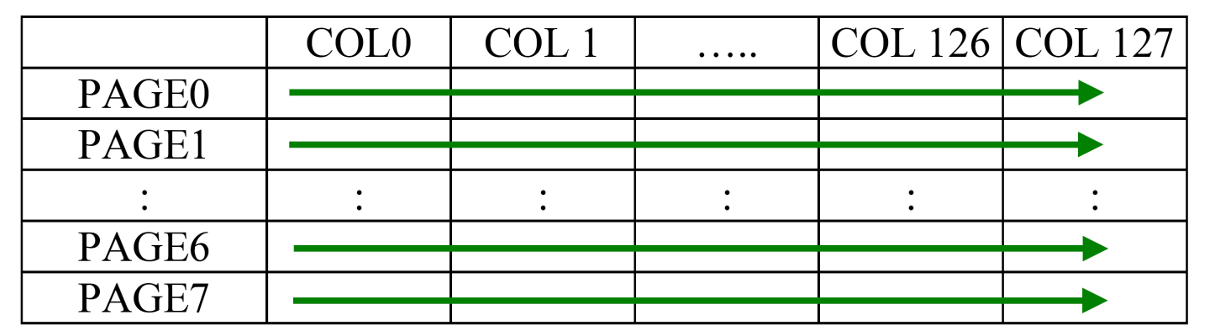
\includegraphics[width=0.7\linewidth]{graphics/address_pointer}
        \caption{Rows and columns of the address memory, with the address pointer movement \cite{SSD1306_Datasheet}}
        \label{fig:addressmemory}
    \end{figure}

    \item \textbf{Memory Location and Character Position:} Each character's position on the screen is determined by its row and column, corresponding to the page and segment in memory. For example, ASCII characters are mapped to the predefined character array, where the ASCII code determines the row in the array, and the bytes represent the visual representation of the character. This mechanism ensures a precise correspondence between memory locations and the screen's display layout.
    \item \textbf{Refreshing the OLED:} The OLED display is periodically refreshed using the TIM3 timer to ensure that updated information is consistently displayed. The \texttt{refresh\_OLED} function is triggered based on the timer's count reaching a predefined threshold of about 4800 counts. Meaning, that the screen must refresh every $\frac{4800}{48000 \text{ Hz}} = 100 \text{ ms}$ \cite{interfacex}. During each refresh cycle, relevant data such as resistance and frequency values are formatted into strings and displayed on specific pages of the OLED screen using the \texttt{oled\_print} function. The timer ensures accurate timing for updates, and the \texttt{TIM3\_delay} function is used to introduce small delays during initialization and resetting processes. This mechanism maintains a responsive and stable display update rate.
        
\end{itemize}

\noindent The designed C module for the OLED screen header and source file is shown in Appendix \ref{sec:oled_screen_c}.




\subsection{Peripheral Justification}
\begin{itemize}
    \item \textbf{ADC/DAC~\cite{interfacex}}: 
        \begin{itemize}
            \item The ADC (12-bit resolution) is crucial for precise analog-to-digital conversion of input signals from the potentiometer.
            \item The DAC enables scalable analog output, supporting external signal generation and circuit testing.
        \end{itemize}
    \item \textbf{TIM2~\cite{iox}}:
        \begin{itemize}
            \item Provides precise timing for frequency measurement by counting clock cycles between signal edges.
            \item Supports high-speed signal processing with overflow detection to ensure robustness in varying signal conditions.
        \end{itemize}
    \item \textbf{GPIO~\cite{iox}}:
        \begin{itemize}
            \item Handles user button inputs and external signal connections.
            \item Configures specific pins (PA0, PA1, PA2) for input signals and mode control.
        \end{itemize}
    \item \textbf{EXTI~\cite{iox}}: 
        \begin{itemize}
            \item Enables hardware-based edge detection for signal frequency measurement.
            \item Critical for capturing precise timing events without CPU intervention, ensuring low-latency performance.
        \end{itemize}
    \item \textbf{OLED Display~\cite{interfacex}}: 
        \begin{itemize}
            \item The SSD1306-based display provides a user-friendly interface to present real-time measurements and system status.
            \item SPI communication ensures efficient data transfer, supporting real-time updates.
        \end{itemize}
\end{itemize}
